%#BIBTEX jbibtex Outline
%\documentstyle[listings,jlisting,txfonts]{grad-abst}

\documentclass[uplatex, 10pt, a4p]{jsarticle}

\usepackage{grad-abst}
\usepackage{listings, jlisting}
\usepackage[dvipdfmx]{graphicx}

\usepackage{verbatim}           % コメントアウトしてくれる便利なプリアンブルが使える \begin{comment} ... \end{comment}
\usepackage{txfonts}
\usepackage{setspace}
\usepackage{url}

\usepackage[dvipdfmx]{hyperref}
\usepackage{pxjahyper} %%hyperref読み込みの直後に

%\addtolength\oddsidemargin{-2.2zw}  % 魔法の呪文01
%\addtolength\evensidemargin{-2.2zw} % 魔法の呪文02
%\addtolength\textwidth{4.4zw}       % 魔法の呪文03

\setcounter{page}{1}

\newcommand{\thesisToolName}{Prot}
\newcommand{\thesisExtensionToolName}{ProtExtension}


\title{OpenModelicaのシミュレーション結果を用いた\\
モータ特性表自動生成ツールの試作}
\author{原田 海人}

\major{情報システム工学科}
\lab{片山(徹)研究室}

%\setstretch{0.9}

%\setlength{\columnseprule}{0.3mm}\setlength{\columnseprule}{0.3mm}

\begin{document}
\maketitle


\section{はじめに}
近年、ソフトウェア開発の効率化が求められており、設計段階や製品を試作する前に、製品の機能や性能を検証したいというニーズが高まっている\cite{modelicaモデルベース本}。
このニーズに応えるために、モデルベースシステム開発手法がある\cite{modelicaモデルベース本}。モデルベースシステム開発手法とは、製品の設計を基にシミュレーションツールを用いて、
シミュレーションを行いながら、設計品質の向上を図る開発手法である\cite{ipa_2016}。この手法は、組込みシステムの開発において特に重要である\cite{ipa_useful_modelbase_dev}。

モデルベースシステム開発手法を用いた組込みシステムの開発には、OpenModelica\cite{open_modelica}が使われる。
OpenModelicaは、Modelica\cite{modelicaモデルベース本}コードのモデリング、シミュレーション、デバッグのための機能などを持つオープンソースプラットフォームである。
OpenModelicaが出力するシミュレーションの結果は、グラフや数値であり、数値においては、csvファイルに出力できる。しかし、この出力を用いて、性能を決定付ける特定の値を確認するためには、手間と時間がかかる。

そこで、本研究では、性能を決定付ける特定の値を確認するためにかかる時間の削減を目的として、OpenModelicaのシミュレーション結果を用いたモータ特性表自動生成ツールの試作を行う。
特性表は、製品の性能をまとめた一覧表であり、複数の製品の性能比較をする際に利用される\cite{特性表1,特性表2,特性表3}。特性表を用いることで、性能の特定の値を容易に確認できるため、本研究の生成対象とする。また、本研究では、ブラシ付きDCモータ\cite{モータ使う}をシミュレーション対象とする。


\section{モータ特性表自動生成ツールの実装}\label{cha:OverviewFunction}
本研究で試作するモータ特性表自動生成ツールの実装について説明する。
試作するモータ特性表自動生成ツールの構造を、図\ref{fig:kouzou}に示す。
試作するモータ特性表自動生成ツールは、OpenModelicaが出力したcsvファイルを入力として受け取り、モータ特性表を生成する。
モータ特性表自動生成機能の処理の流れを、以下に示す。
\begin{enumerate}
    \item 実行コマンドを取得する
    \item 第1引数で指定されたcsvファイルを読み込む
    \item 第2引数、第3引数で指定したモジュール名が持つデータを、csvファイルから取得する
    \item モータ特性表の各要素を算出する
    \item 特性表を作成する
    \item 特性グラフを作成する
    \item モータ特性表を生成する
\end{enumerate}
\begin{figure}[tp]
	\centering
	\fbox{
    \includegraphics[width=\columnwidth]{./Image/Kouzou.png}
    }
    \caption{試作したモータ特性表自動生成ツールの構造}
	\label{fig:kouzou}
\end{figure}
試作したモータ特性表自動生成ツールが生成するモータ特性表の例を、図\ref{fig:chtable}に示す。

特性表とは、以下の12個の値で構成する。
% \begin{itemize}
% 	\item 電圧 V
% 	\item 始動電流 mA
% 	\item 停動トルク $mN \cdot m$
% 	\item 最大効率 \%
% 	\item 定格トルク $mN \cdot m$
% 	\item 定格回転数 rpm
% 	\item 定格電流 mA
% 	\item 定格出力 W
% 	\item 最大回転数 rpm
% \end{itemize}
% 以下に各要素が表す内容について述べる。
\begin{itemize}
\item{定格電圧(Rated Voltage)}
% \\item{電圧}\label{sub:dennatu}\\
定格電圧とは、モータが回転する電圧の基準値を表す。本研究では、シミュレーション時に回路に印加した電圧値を定格電圧とする。

単位は、$\mathrm{V}$である。
\item{始動電流(Starting Current)}\label{sub:sub:sidouden}
% \\item{始動電流}\label{sub:sidouden}
始動電流とは、モータを始動する際、回路に流れる電流の最大値を表す。

単位は、$\mathrm{mA}$である。
% https://www.tsugawa.co.jp/glossary/ 

\item{無負荷電流(No-Load Current)}
無負荷電流とは、モータに負荷がかかっていないときの電流値を表す。

単位は、$\mathrm{mA}$である。

\item{無負荷回転数(No-Load Speed)}
無負荷回転数とは、モータに負荷がかかっていないときの回転数を表す。

単位は、$\mathrm{rpm}$である。

\item{始動トルク(Starting Torque)}
始動トルクとは、モータが始動する際に発生するトルクの値を表す。

単位は、$\mathrm{mN \cdot m}$である。


\item{停動トルク(Stalling Torque)}\label{sub:sub:teidoutoruku}
% \\item{停動トルク}\label{sub:teidoutoruku}
% 停動トルクとは、モータが出しうる最大トルクで、このトルク以上の負荷がかかれば、モータが停止する値を表す。
停動トルクとは、モータが停止する負荷トルクの値を表す。負荷トルクとは、モータの回転を停止させようとする力のことである。

単位は、$\mathrm{mN \cdot m}$である。

% https://www.orientalmotor.co.jp/tech/glossary/ta11/
\item{最大効率(Maximum Efficiency)}\label{sub:sub:saidaikouritu}
% \\item{最大効率}\label{sub:saidaikouritu}
最大効率とは、効率の最大値を表す値である。効率とは、モータに与える入力エネルギーとモータを回転させるために要した機械エネルギーの比を百分率[\%]で表した値である。入力エネルギーは電流と電圧の積で計算でき、出力エネルギーはモータの回転に加わるトルクと角速度で計算できる。効率を算出する式を、以下に示す。

\[
    \mbox{出力} = \mbox{角速度} \times \mbox{トルク}
\]
\[
    \mbox{入力} = \mbox{電圧} \times \mbox{電流}
\]

\[
    \mbox{効率} = \frac{\mbox{出力}}{\mbox{入力}}  \times 100
\]

単位は、$\mathrm{\%}$である。
% https://www.jp-igarashi.com/product/product_motors/curve.html
\item{定格トルク(Rated Torque)}\label{sub:sub:teikakutoruku}
% \\item{定格トルク}\label{sub:teikakutoruku}
定格トルクとは、最大効率時のトルク値を表す。

単位は、$\mathrm{mN \cdot m}$である。
% http://www.sagamimicro.co.jp/product/aboutusage.html
\item{定格回転数(Rated Speed)}\label{sub:sub:teikakukaiten}
% \\item{定格回転数}\label{sub:teikakukaiten}
定格回転数とは、最大効率時のモータの回転数の値を表す。

単位は、$\mathrm{rpm}$である。

% https://mathwords.net/kaitensu
\item{定格電流(Rated Current)}\label{sub:sub:teikakuden}
% \\item{定格電流}\label{sub:teikakuden}
定格電流とは、最大効率時の電流値を表す。

単位は、$\mathrm{mA}$である。
% http://fa-faq.mitsubishielectric.co.jp/faq/show/18504?category_id=1937&site_domain=default
\item{定格出力(Rated Power)}\label{sub:sub:teikakusyutu}
% \\item{定格出力}\label{sub:teikakusyutu}
定格出力とは、最大効率時の出力値を表す。
定格出力を計算する式を、以下に示す。
\[  \mbox{定格出力} = \mbox{定格トルク} * \mbox{定格回転数} * \frac{2\pi}{60} \]
単位は、$\mathrm{W}$である。
% \ref{sub:sub:teikakukaiten}章で求めた定格回転数と\ref{sub:sub:teidoutoruku}章で求めた定格トルクを
% http://www.nidec-servo.com/jp/digital/pdf/A_technique.pdf
\item{最大回転数(Maximum Speed)}\label{sub:sub:saidaikai}
% \\item{最大回転数}\label{sub:saidaikai}
最大回転数とは、回転数の値の中で最大値を表す。

\end{itemize}




\begin{figure}[t]
	\centering
	\fbox{
    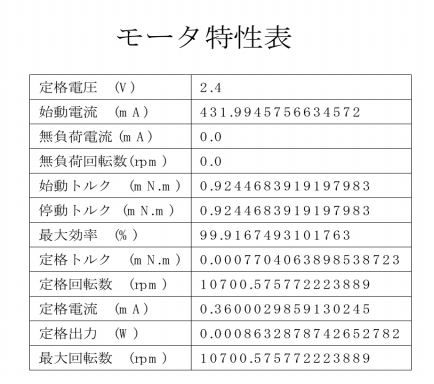
\includegraphics[width=\columnwidth]{./Image/chta_small.png}
    }
    \caption{試作したツールが生成する特性表の例}
	\label{fig:chtable}
\end{figure}

\section{適用例}\label{sec:Indication}
本章では、本研究で作成したモータ特性表自動生成ツールが正しく動作することを確認する。
ブラシ付きDCモータのModelicaモデルが出力するcsvファイルに対して、本研究で試作したモータ特性表自動生成ツールを適用した結果を、図\ref{fig:tekiyou_mortoku}に示す。図\ref{fig:tekiyou_mortoku}により、OpenModelicaモデルが出力したcsvファイルかモータ特性表を生成できていることが確認できる。

\begin{figure}[t]
	\centering
	\fbox{
    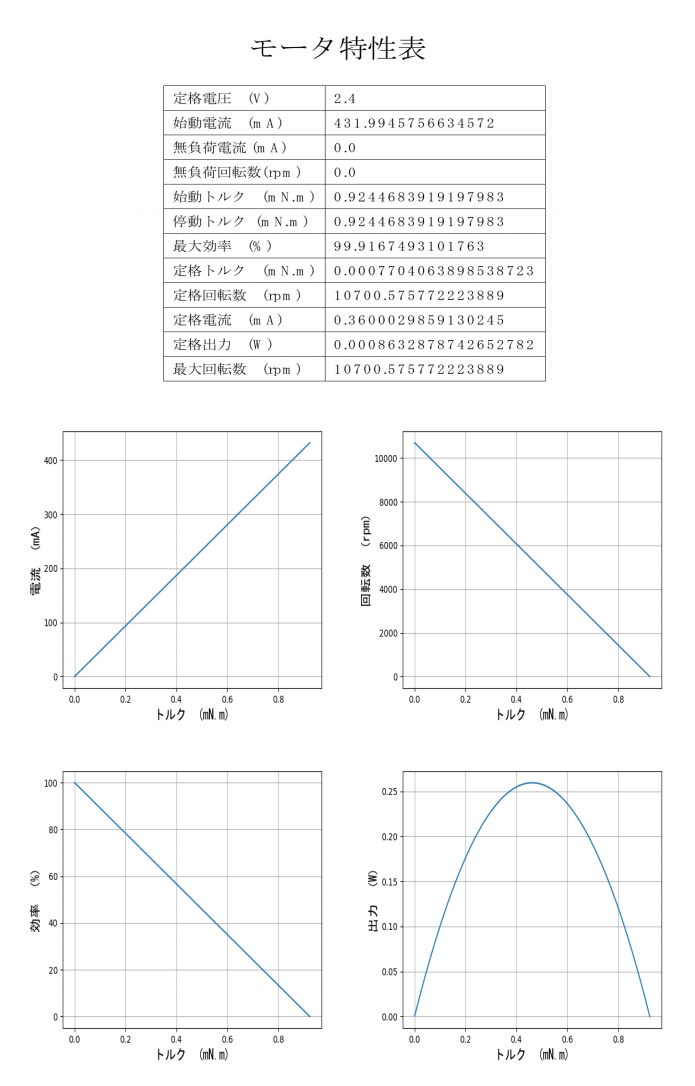
\includegraphics[width=\columnwidth]{./Image/kakunin_chta1.png}
    }
    \caption{適用例で生成したモータ特性表}
	\label{fig:tekiyou_mortoku}
\end{figure}

\section{考察}\label{sec:Evaluation}
本論文で試作したモータ特性表自動生成ツールの有用性を評価するため、本研究室の学部4年生4人に対して、実験を行い、特定の値を確認するためにかかる時間を削減できたかどうかを検証する。
実験には、内容が異なる2つのシミュレーション結果のcsvファイルを用いた。これらのcsvファイルをそれぞれ「ファイルA」、「ファイルB」と定義する。

実験方法は、ケースXとケースYに分けて行う。

ケースXでは、ファイルAに対して、モータ特性表自動生成ツールを用いず、表計算ソフトを用いて問題に解答してもらう。次に、ファイルBに対して、モータ特性表自動生成ツールを用いて問題に解答してもらう。

ケースYでは、ファイルBに対して、モータ特性表自動生成ツールを用いず、表計算ソフトを用いて問題に解答してもらう。次に、ファイルAに対して、モータ特性表自動生成ツールを用いて問題に解答してもらう。

ケースXとケースY で出題する問題を、図\ref{fig:mondai}に示す。

この問題を解答するのに要する時間を測定することにより、モータ特性表自動生成ツールを用いることで、特定の値を確認するためにかかる時間を削減できるかどうかを検証する。

被験者4名を2つのグループに分け、片方のグループに「ケースX」の実験を行い、もう片方のグループに「ケースY」の実験を行った。

「ケースX」の実験結果を表\ref{resultX}に、「ケースY」の実験結果を表\ref{resultY}に、それぞれ示す。これらの実験結果より、モータ特性表自動生成ツールを用いた場合、用いなかった場合に比べて、解答に要する時間を平均で、「91.95」\%削減できた。また、モータ特性表自動生成ツールを用いた場合の方が、用いなかった場合に比べて正答率が高いことが示せた。よって本研究で試作したモータ特性表自動生成ツールを用いることで、性能を決定づける特定の値を確認するためにかかる時間を削減できると言える。

%TODO 問題文にしよう!
\begin{figure}[tp]
	\centering
	\fbox{
	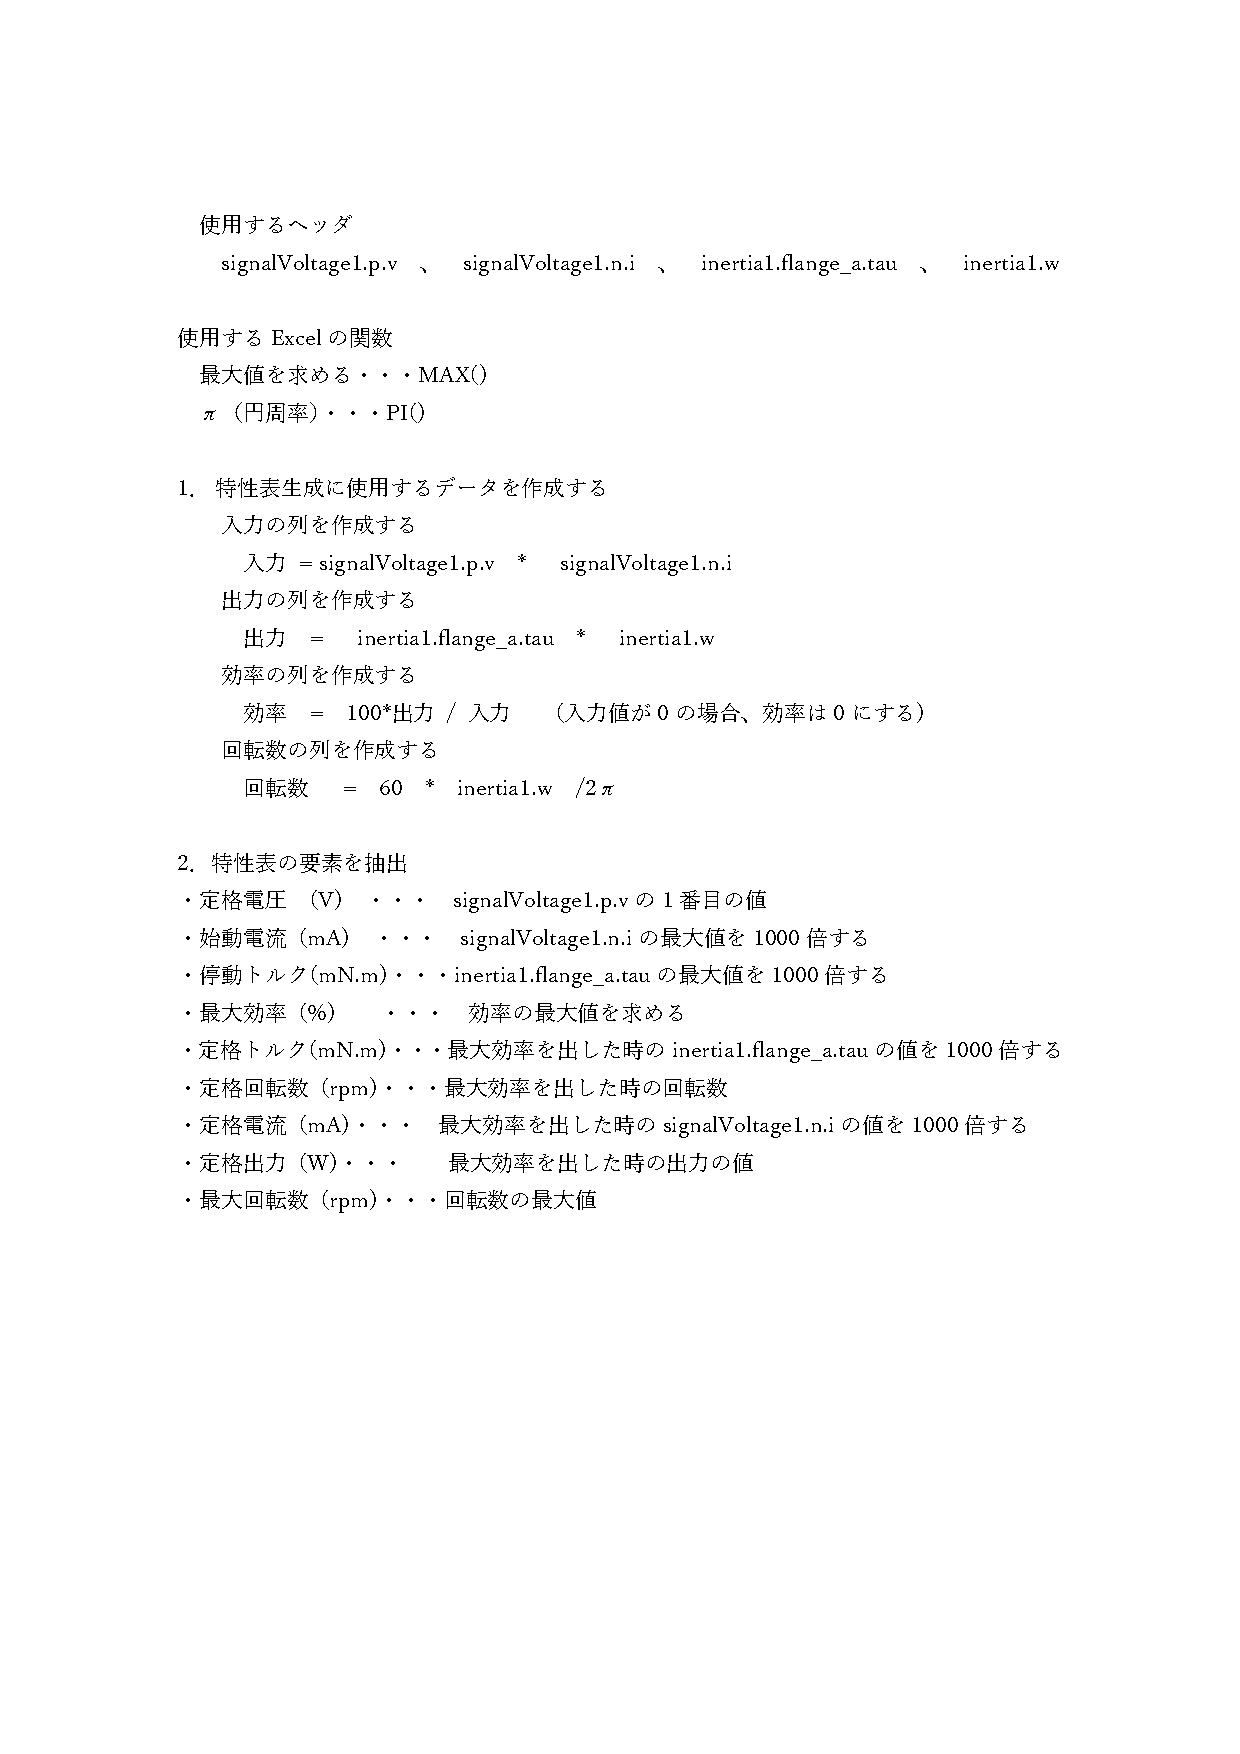
\includegraphics[width=8cm,pagebox=cropbox]{Image/実験方法の説明.pdf}
	}
	\caption{ケースXとケースY で出題する問題}
	\label{fig:mondai}
\end{figure}

\begin{table}[tp]
  \begin{center}
    \caption{ケースXの実験結果}
    \label{resultX}
    \begin{tabular}{c|c|c|c|c|}
    \cline{2-5}
                              & \multicolumn{2}{c|}{ツール未使用} & \multicolumn{2}{c|}{ツール使用} \\ \hline
    \multicolumn{1}{|c||}{被験者} & 解答時間           & 正答率          & 解答時間           & 正答率         \\ \hline\hline
    \multicolumn{1}{|c||}{1}   & 13分5秒           & 56\%         & 57秒           & 100\%         \\ \hline
    \multicolumn{1}{|c||}{2}   & 14分50秒          & 67\%          & 1分20秒          & 100\%         \\ \hline\hline
    \multicolumn{1}{|c||}{平均}   & 13分57.5秒          & 61.5\%          & 1分8.5秒          & 100\%         \\ \hline
    \end{tabular}
  \end{center}
\end{table}

\begin{table}[tp]
  \begin{center}
    \caption{ケースYの実験結果}
    \label{resultY}
    \begin{tabular}{c|c|c|c|c|}
    \cline{2-5}
                              & \multicolumn{2}{c|}{ツール未使用} & \multicolumn{2}{c|}{ツール使用} \\ \hline
    \multicolumn{1}{|c||}{被験者} & 解答時間           & 正答率          & 解答時間           & 正答率         \\ \hline\hline
    \multicolumn{1}{|c||}{3}   & 21分35秒           & 67\%         & 1分10秒           & 100\%         \\ \hline
    \multicolumn{1}{|c||}{4}   & 18分6秒          & 100\%          & 1分58秒          & 89\%         \\ \hline\hline
    \multicolumn{1}{|c||}{平均}   & 19分50.5秒          & 83.5\%          & 1分34秒          & 94.5\%         \\ \hline
    \end{tabular}
  \end{center}
\end{table}

\section{おわりに}
本論文では、性能を決定付ける特定の値を確認するためにかかる時間の削減を目的として、OpenModelicaのシミュレーション結果を用いたモータ特性表自動生成ツールを試作した。
なお、本研究では、シミュレーションの対象として、ブラシ付きDCモータを対象とする。

モータ特性表自動生成ツールは、csvファイル解析部、特性表の要素算出部、モータ特性表生成部の3つの処理部で構成している。
csvファイル解析部では、csvファイルを読み込み、モータ特性表を生成するために必要なデータを抽出する。特性表の要素算出部では、抽出したデータからモータ特性表の各要素を算出する。
モータ特性表生成部では、算出した各要素を基に、特性表と4つの特性グラフを生成し、これらを1つのPDFファイルにまとめ、モータ特性表として出力する。

適用例として、ブラシ付きDCモータのModelicaモデルのシミュレーション結果であるcsvファイルを用いる。このcsvファイルを試作したモータ特性表自動生成ツールに適用した結果、正しくモータ特性表を生成することを確認した。

考察において、モータ特性表自動生成ツールの有用性を示すことができた。具体的には、モータ特性表自動生成ツールを用いることにより、性能の特定の値を確認するためにかかる時間を削減できることを検証した。
検証にはケースXとケースYの2種類のケースを用意し、被験者4名を2グループに分けて、モータ特性表自動生成ツールを用いる場合と、用いない場合で実験を行った。

これらの実験結果より、モータ特性表自動生成ツールを用いた場合、用いなかった場合に比べて、解答に要する時間の平均を、91.95\%削減できた。また、モータ特性表自動生成ツールを用いた場合の方が、用いなかった場合に比べて、正答率が高かった。


% この実験結果により、ケースXについてはモータ特性表自動生成ツールを使用した場合では、使用しなかった場合に比べて被験者の回答時間を91.8\%削減できた。
% ケースYについては、モータ特性表自動生成ツールを使用した場合では、使用しなかった場合に比べて被験者の回答時間を92.1\%削減できた。
% この結果により、モータの性能を決定づける特定の値を確認するためにかかる時間を削減できたと言える。また、双方のケースにおいて、モータ特性表自動生成ツールを用いた場合、モータ特性表自動生成ツールを用いない場合に比べ、問題の正答率が上昇した。
% 正答率が上がった理由として、モータ特性表自動生成ツールを用いる
% 人手によるミスを削減できたことが考えられる。具体的には、モータ特性表自動生成ツールを用いない場合、手動で表計算ソフトから特定の値を抽出し、計算を行う必要があるため、
% この過程においてミスが発生する可能性が高まったことが考えられる。
% 一方、モータ特性表自動生成ツールを用いた場合、ツールが自動で特性表を生成し、提示することにより、人手によるミスが発生する可能性を削減できたことが考えられる。

以下に、今後の課題を示す。

\begin{itemize}
    \item 対象とするモータのモデルが1種類しかない\\
    本論文で試作したモータ特性表自動生成ツールが対象とするのはブラシ付きDCモータである。しかし、ブラシレスモータやACモータなどには対応していない。
    そのため、それらを用いた回路のシミュレーション結果からモータ特性表を作成できない。

\item 特性表の要素をユーザが変更できない\\
      本論文で試作したモータ特性表自動生成ツールが生成する特性表は、12個の要素を持つ。
      しかし、ユーザがこの要素を変更することはできない。

\end{itemize}

%\footnotesize
\bibliography{bibtex} %bibファイルの.bibの前の部分


\bibliographystyle{junsrt} %引用された順番に出力
\end{document}

